\section{The Exponential Decay Problem}

\par We would like a simple toy problem with which we can build a framework for the analysis of the stability of a numerical method.\\
We turn to a classic problem in numerical analysis: the Exponential Decay Problem.\\
Consider a quantity $y$ that decays relative to its current value.\\
The quantity at time $t$ is $y(t)$ and the rate of decay is $\lambda$.\\
For the solution to actually decay, we require $Re(\lambda) < 0$.\\

\par The Exponential Decay Problem is given by the ODE
\[y'(t) = \lambda y(t) \quad \text{with} \quad y(0) = y_0\]
This has the exact solution $y(t) = y_0\, e^{\lambda t}$, hence the name 'Exponential Decay'.\\

\par For the sake of keeping things neat, we will take $y_0 = 1$ for the rest of this paper.\\
This poses no lack of generality, as we can always scale the solution by any initial value, both exact and numerical.\\

\par The exact solution we will consider is \[y(t) = e^{\lambda t}\]\\

\subsection{A Graphical Representation}
Appendix~\ref{appendix:exact} contains the Python for these graphs.
\begin{multicols}{2}
\begin{center}
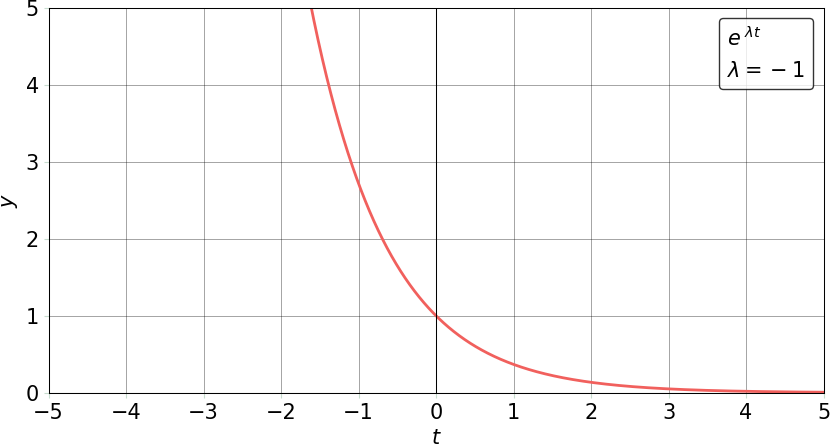
\includegraphics[width=0.4\textwidth]{Exponential Decay/Exact with -1.png}
\end{center}
\par \hspace*{1cm} If we restrict $\lambda$ to $\bR^{-}$, we have a simple\\
\hspace*{1cm} exponential curve that decays to zero as $t \rightarrow \infty$.\\
\columnbreak{}
\begin{center}
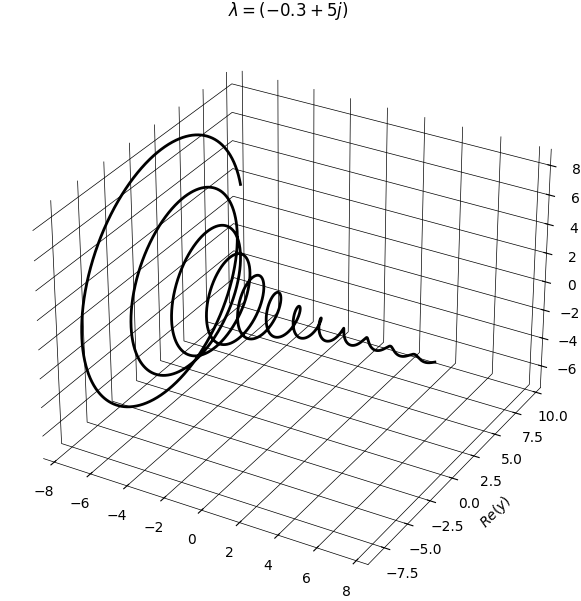
\includegraphics[width=0.4\textwidth]{Exponential Decay/Exact with (-0.3+5j).png}
\end{center}
\par \hspace*{1cm} If we allow $\lambda \in \bC$ and $Re(\lambda)<0$,\\
\hspace*{1cm} we get a spiral in the complex plane,\\
\hspace*{1cm} the radius of which decays to zero as $t \rightarrow \infty$.\\
\end{multicols}

\subsection{The Maclaurin Series}
The Taylor series is given by:
\[y(t) = \sum\limits_{n=0}^{\infty} \frac{{y}^{(n)}(a)}{n!}{(t-a)}^n\]
Setting $a=0$, we get the Maclaurin series for the exact solution:
\[y(t) = \sum\limits_{n=0}^{\infty} \frac{{(\lambda)}^n e^0}{n!}t^n = \sum\limits_{n=0}^{\infty} \frac{{(\lambda t)}^n}{n!} \quad\text{which we will denote}\; M(y)\]
This is a useful form for the exact solution -- we will see it pop up again later.

\subsection{Proponents of the Exponential Decay Problem}
\par There are a few pros to this choice of problem:
\begin{itemize}
    \item[$\cdot$] The exact solution is known and easily computed; it can be used to evaluate a numerical solution.
    \item[$\cdot$] The solution is a straightforward and well understood function.\\
    	  This simplicity allows us to focus on the numerical method.
    \item[$\cdot$] The problem is linear in $y(t)$, making the problem simple to work with.\\
    	  Again, our focus can stay on the numerical method.
    \item[$\cdot$] The graph of the exact solution is easy to visualise; the more chaotic outputs of the numerical methods can be compared to the smooth curve of the exact solution easily.
    \item[$\cdot$] Exponential decay is a model for many physical processes, including radioactive decay, population decline, and capacitor discharge.\\
    	  Quantities that decay relative to their current value appear frequently in nature.\\
    	  This means readers from many different disciplines may already possess an intuition for the problem.
    \item[$\cdot$] The problem is simple to generalise to complex numbers, allowing us to explore the stability of numerical methods in the complex plane.
    \item[$\cdot$] The Exponential Decay Problem is \term{stiff}; for certain method-step pairs, the numerical solution may oscillate wildly.\\
    	  This is exactly the kind of behaviour we want to avoid in a numerical method, when we are looking for stability.
\end{itemize}

\par Normally, when using the Exponential Decay Problem in a numerical analysis context, we would allow $\lambda \in \bC$ with $Re(\lambda)<0$.\\
However, for the purposes of this paper, we will restrict $\lambda$ to $\bR$ as we will be looking at $h \in \bC$ and we don't want to overcomplicate things.\\
Unless otherwise mentioned, we will assume that $\lambda \in \bR^{-}$ for the rest of this paper.\\

\par We will use the Exponential Decay Problem throughout this paper to derive a useful framework for the analysis of the stability of a numerical method.\\
